\subsection{Field Strength Renormalization}
we can use the spectrol of interacting hamitonian H to create a identity operator,since H is commute with the total momentum P,we can choose the states with:
\[\diracr{\Omega},\diracr{\lambda_0},\diracr{\lambda_p}\]
where the relations is:
\[H\diracr{\Omega}=0\diracr{\Omega},P\diracr{\Omega}=0\diracr{\Omega}\]
\[H\diracr{\lambda_0}=E_0\diracr{\lambda_0}=m_\lambda\diracr{\lambda_0},P\diracr{\lambda_0}=0\diracr{\lambda_0}\]
\[H\diracr{\lambda_p}=E_p\diracr{\lambda_p},P\diracr{\lambda_p}=p\diracr{\lambda_p}\]
where,
\[E_p=\sqrt{|\vec{p}|^2+m_\lambda^2}\]
since the state with total momentum zero is not only one,so different $\lambda$ give the different such states;\par
then we can use there states to construct the identity operotor:
\[1=\diracr{\Omega}\diracl{\Omega}+\sum_\lambda\int\frac{d^3p}{(2\pi)^3)}\frac{1}{2E_\lambda}\diracr{\lambda_p}\diracl{\lambda_p}\] 
insert this operotor into the correction function one can get:
\[\diracl{\Omega}\phi(x)\phi(y)\diracr{\Omega}=\sum_\lambda\int\frac{d^4p}{(2\pi)^4)}\frac{i}{p^2-m_\lambda^2+i\epsilon}|\diracl{\Omega}\phi(0)\diracr{\lambda_0}|^2\]
so we have dervied the Kallen-Lehmann spectral representation of the two-points function:
\[\diracl{\Omega}T\phi(x)\phi(y)\diracr{\Omega}=\int \frac{dM^2}{2\pi}\rho(M^2)D_F(x-y,M^2)\]
and the general form for $\rho(M^2)$ is:
\[\rho(M^2)=\sum_{\lambda} 2\pi\delta(M^2-m_\lambda^2)|\diracl{\Omega}\phi(0)\diracr{\lambda_0}|^2\]
\[\rho(M^2)=2\pi\delta(M^2-m_\lambda^2)Z+nothing-untill- M^2\gtrsim (2m)^2\]
we call Z as the \textcolor{red}{field strength renormalization}\par
and the fourier transfer of the two points function is:
\[\int d^4xe^{ipx}\diracl{\Omega}T\phi(x)\phi(0)\diracr{\Omega}=\frac{iZ}{p^2-m^2+i\epsilon}+\int_{\sim 4m^2}^\infty\frac{dM^2}{2\pi}\rho(M^2)\frac{i}{p^2-M^2+i\epsilon}\] 
and for the dirac firld,the quantity is:
\[\int d^4xe^{ipx}\diracl{\Omega}T\psi(x)\bar{\psi}(0)\diracr{\Omega}=\frac{iZ(\slashed{p}+m)}{p^2-m^2+i\epsilon}+\cdots\]
\subsection{The LSZ reduction formula}
Lehmann,Symanzik,Zimmerman;\par
\begin{align*}
&\prod_1^n\int d^4x_ie^{ip_ix_i}\prod_1^m\int d^4y_je^{-ik_jy_j}\diracl{\Omega}T\{\phi(x_1)\cdots\phi(x_n)\phi(y_1)\cdots\phi(y_m)\}\diracr{\Omega}\\
&\sim_{p_i^0\rightarrow +E_{\vec{p}_i},k_j^0\rightarrow +E_{\vec{k}_j}}=(\prod_1^n\frac{i\sqrt{Z}}{p_i^2-m^2+i\epsilon})(\prod_1^m\frac{i\sqrt{Z}}{k_j^2-m^2+i\epsilon})\diracl{p_1\cdots p_n}S\diracr{k_1\cdots k_m}
\end{align*}
using LSZ reduction formula,one can work out the feymann diagrammatic method for the  S metrics elements \ref{fig:amputa}
\begin{figure}
\begin{center}
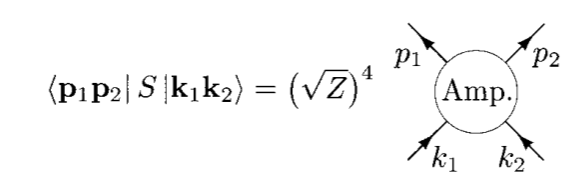
\includegraphics[height=4cm]{./figures/AmputatedFey}
\caption{Using LSZ formula to calculate the S metrics elements.}
\label{fig:amputa}
\end{center}
\end{figure}
\subsection{The Optical Theorem}
since 
\[S^{\dagger}S=1\]
on can get the result:
\[-i[T-T^{\dagger}]=T^{\dagger}T\]
insert a complete set of intermedia states one can get:
\begin{align*}
&-i[M(k_1k_2\rightarrow p_1p_2)-M^*(p_1p_2\rightarrow k_1k_2)]
\\
&=\sum_n(\prod_{i=1}^n\int \frac{d^3q_i}{(2\pi)^3}\frac{1}{2E_i})M^*(p_1p_2\rightarrow \{q_i\})M(k_1k_2\rightarrow\{q_i\})\times(2\pi)^4\delta^{(4)}(k_1+k_2-\sum_iq_i)
\end{align*}
so one can get the optical theorem:
\[2Im M(k_1k_2\rightarrow k_1k_2)=2E_{cm}p_{cm}\sigma_{tot}(k_1k_2\rightarrow anything)\]
\subsection{The Ward-Takahashi Identity}
the warden identity is illustated in figure \ref{fig:warden}.\par Ward identity is the diagrammatic expression of the current conservation,which is in turn a consequence of gauge invariance\par
\begin{figure}
\begin{center}
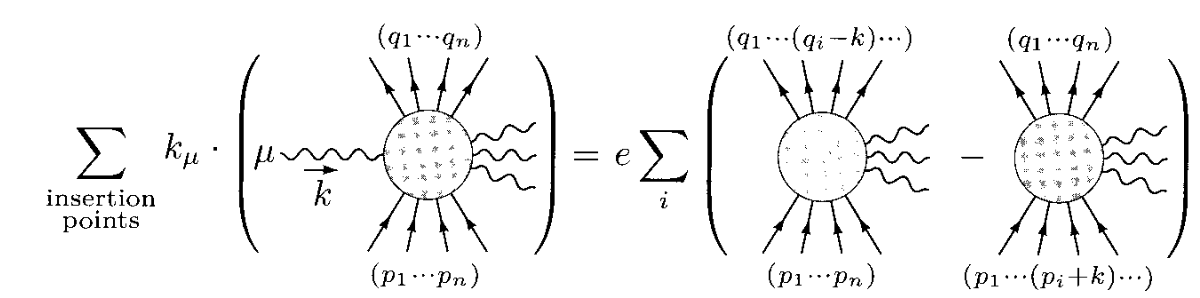
\includegraphics[height=4cm]{figures/warden}
\caption{The Ward-Takahashi Identity}
\label{fig:warden}
\end{center}
\end{figure}

\subsection{Renormalization of the Electric Charge}
the definition and diagram is illustrated as figure \ref{fig:loop1} and \ref{fug:loop2}。from the ward identity ,one can expect the form:\par
\begin{figure}
\begin{center}
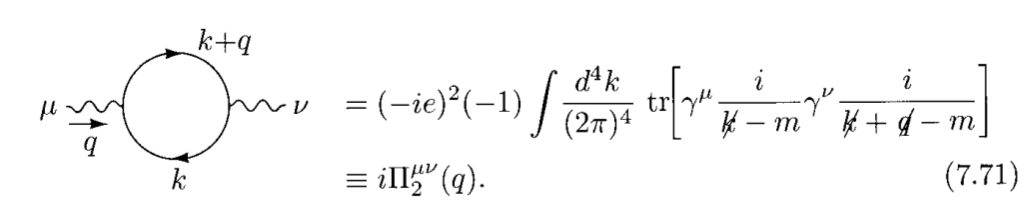
\includegraphics[height=3cm]{figures/loop1}
\caption{The feymann diagram for loop}
\label{fig:loop}
\end{center}
\end{figure}
\begin{figure}
\begin{center}
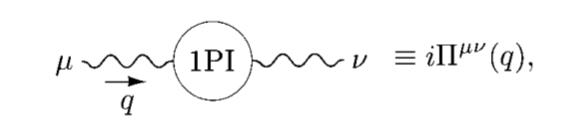
\includegraphics[height=3cm]{figures/loop2}
\caption{The 1PI Part}
\label{fig:loop2}
\end{center}
\end{figure}
\[\Pi^{\mu\nu}(q)=(q^2g^{\mu\nu}-q^\mu q^\nu)\Pi(q^2)\]
thus the calculation result is as the figure \ref{fig:loop3} shows.
\begin{figure}
\begin{center}
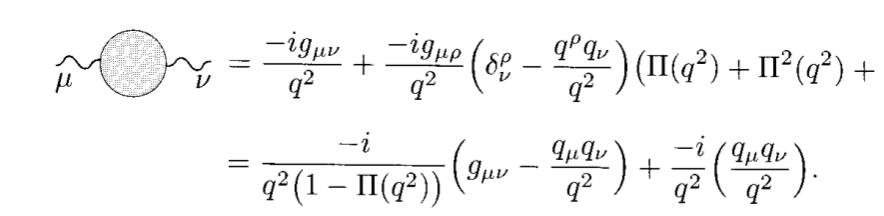
\includegraphics[height=3cm]{figures/loop3}
\caption{the result of the above digram}
\label{fig:loop3}
\end{center}
\end{figure}
\begin{figure}
\begin{center}
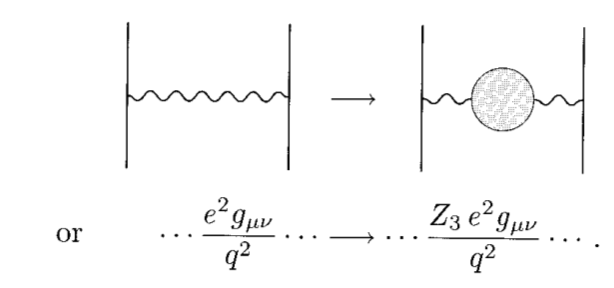
\includegraphics[height=5cm]{figures/loop4}
\caption{the charge regulization}
\label{fig:loop4}
\end{center}
\end{figure}
where the $Z_3$ is called charge regulization:
\[Z_3=\frac{1}{1-\Pi(0)}\]
\[e_0\rightarrow \sqrt{Z_3}e_0\]
after a long journey of calculation using feymann parameter, wick rotation ,one can work out:
\[i\Pi_2^{\mu\nu}(q^2)=-4ie^2\int _0^1dx\int\frac{d^4 l_E}{(2\pi)^4}\frac{\frac{1}{2}l_E^2g^{\mu\nu}-2x(1-x)q^\mu q^\nu+g^{\mu\nu}(m^2+x(1-x)q^2)}{(l_E^2+\Delta)^2}\]
with:
\[\Delta=m^2-x(1-x)q^2\]
which is baddly ultraviolet divergent. and voilate the ward identity.\par
\subsection{Dimennsional Regularization}
The area of a d dimensional unit sphere is:
\[\int d\Omega_d=\frac{2\pi^{\frac{d}{2}}}{\Gamma(\frac{d}{2})}\]
and one can work out the d-dimensional integration using gamma and beta function:
\[\int \frac{d^dl_E}{(2\pi)^d}\frac{1}{(l_E^2+\Delta)^2}=\frac{1}{(4\pi)^{\frac{d}{2}}}\frac{\Gamma(2-\frac{d}{2})}{\Gamma(2)}(\frac{1}{\Delta})^{2-\frac{d}{2}}\]
then we take the limit $d\rightarrow 4$ since:
\[\Gamma(2-\frac{d}{2})=\Gamma(2-\frac{4-\epsilon}{2})=\Gamma(\frac{\epsilon}{2})=\frac{2}{\epsilon}-\gamma+O(\epsilon)\]
then the above integration is:
\[\int \frac{d^dl_E}{(2\pi)^d}\frac{1}{(l_E^2+\Delta)^2}=_{d\rightarrow 4}=\frac{1}{(4\pi)^2}(\frac{2}{\epsilon}-\ln \Delta-\gamma+\ln(4\pi)+O(\epsilon))\]
similarly:
\[\int \frac{d^dl_E}{(2\pi)^d}\frac{1}{(l_E^2+\Delta)^n}=\frac{1}{(4\pi)^{\frac{d}{2}}}\frac{\Gamma(n-\frac{d}{2})}{\Gamma(n)}(\frac{1}{\Delta})^{n-\frac{d}{2}}\]
\[\int \frac{d^dl_E}{(2\pi)^d}\frac{l_E^2}{(l_E^2+\Delta)^n}=\frac{1}{(4\pi)^{\frac{d}{2}}}\frac{d}{2}\frac{\Gamma(n-\frac{d}{2}-1)}{\Gamma(n)}(\frac{1}{\Delta})^{n-\frac{d}{2}-1}\]
in d dimensional space:
\[g^{\mu\nu}g_{\nu\mu}=d\]
\[l^\mu l^\nu-\rightarrow \frac{1}{d}l^2g^{\mu\nu}\]
the dirac metric becomes a set of d metrics:
\[\{\gamma^\mu,\gamma^\nu\}=2g^{\mu\nu},tr[1]=4\]
\[\gamma^\mu\gamma^\nu\gamma_\mu=-(2-\epsilon)\gamma^\nu\]
\[\gamma^\mu\gamma^\nu\gamma^\rho\gamma_\mu=4g^{\nu\rho}-\epsilon\gamma^\nu\gamma^\rho\]
\[\gamma^\mu\gamma^\nu\gamma^\rho\gamma^\sigma\gamma_\mu=-2\gamma^\sigma\gamma^\rho\gamma^\nu+\epsilon \gamma^\nu\gamma^\rho\gamma^\sigma\]
after a long journey of calculation one can work out:
\[i\Pi_2^{\mu\nu}(q)=(q^2g^{\mu\nu}-q^\mu q^\nu)i\Pi_2(q^2)\]
with,
\[\Pi_2(q^2)=\frac{-8e^2}{(4\pi)^{\frac{d}{2}}}\int_0^1dx x(1-x)\frac{\Gamma(2-\frac{d}{2})}{\Delta^{2-\frac{d}{2}}}\]
\[\Pi_2(q^2)\sim_{d\rightarrow 4}=-\frac{2\alpha}{\pi}\int_0^1dx x(1-x)(\frac{2}{\epsilon}-\ln \Delta-\gamma+\ln(4\pi)+O(\epsilon))\]
\[V(r)=-\frac{\alpha}{r}(1+\frac{\alpha}{4\sqrt{\pi}}\frac{e^{-2mr}}{(mr)^{\frac{3}{2}}}+\cdots)\]
the rediative correction term is called Uehling Potential.\par
